\documentclass[journal]{IEEEtran}
\usepackage{cite}
\usepackage[dvips]{graphicx}
\usepackage{hyperref}
\graphicspath{{/home/joaquin/Dropbox/figures/diagrams/}{/home/joaquin/Dropbox/figures/}{/home/joaquin/Dropbox/python/figures/}{/home/joaquin/Dropbox/figures/eps/}}

\begin{document}
\title{150 ps all-optical switching in silicon microring resonators}
\author{J.~Matres, J.~Marti and~C.~J.~Oton}
\markboth{IEEE PHOTONICS TECHNOLOGY LETTERS}{Shell \MakeLowercase{\textit{J. Matres et al.}}: 150 ps all-optical switching in silicon microring resonators}
\maketitle

\begin{abstract}
We present the ultrafast nonlinear characterization of a CMOS-compatible silicon waveguide. A phase sensitive pump and probe technique was implemented in order to monitor the phase and amplitude response of the system with 1 picosecond resolution. This allowed the characterization of carrier generation and recombination dynamics, where decay times below 150~ps were observed. With this device, we show an all-optical modulator based on an integrated microring resonator with 10~dB extinction and 1/e recovery time of 150~ps.
\end{abstract}

\section{Introduction}
Integrated silicon-based optical devices have recently emerged as a feasible technology to route, switch and modulate signals in optical networks, which are expected to dramatically reduce device costs and provide new functionalities \cite{Soref2006}. However the main limitation in these devices is that ultrafast effects, such as Kerr, require so high powers that free-carriers are generated through two-photon absorption (TPA), limiting the speed of commutators \cite{Oton}, logic gates \cite{Oton2010}, etc.
To solve this limitation there are several techniques to sweep this carriers, the most common  of them is to create a reverse biased PN junction \cite{Turner-Foster2010}.
In this work we present two different nonlinear experiments to characterize the dynamics of nonlinear effects such as Kerr, cross absorption modulation and free-carrier dispersion. In the first experiment we will observe the phase and amplitude response of high power pulses (pump) over low power pulses (probe). The other experiment is optical switching; it is also based on controlling a low-power signal (probe), through high power pulses (pump).

 
\section{Fabrication}
The samples used were fabricated from SOI wafers with 3~$\mu m$ buried oxide and 250~nm silicon layer. The waveguides were patterned with e-beam lithography and etched with an inductively coupled plasma (ICP) etcher. The structures were covered with 2~$\mu m$ of silica after SEM characterization. The channels are 500~nm wide and 250~nm high, and are coupled to 20~$\mu m$-radius rings through a 300~nm gap. Light was coupled into the waveguides by butt-coupling with lensed fibers, and was extracted with an objective. The TM transmission spectrum was measured by tuning the laser, and the result is shown in Fig.~\ref{fig:fit20um300nmBig}, where one resonance is shown. The response was fitted to the theoretical equation~\cite{heebner2007optical} by using the propagation loss and coupling coefficient as parameters. A good agreement was found for propagation loss of 20~dB/cm and coupling coefficient k = 0.072. Full width at half depth (FWHD) of the peak was 92~pm, which corresponds to a Q-factor of 16870. 


\begin{figure}[htb]
    \centering
    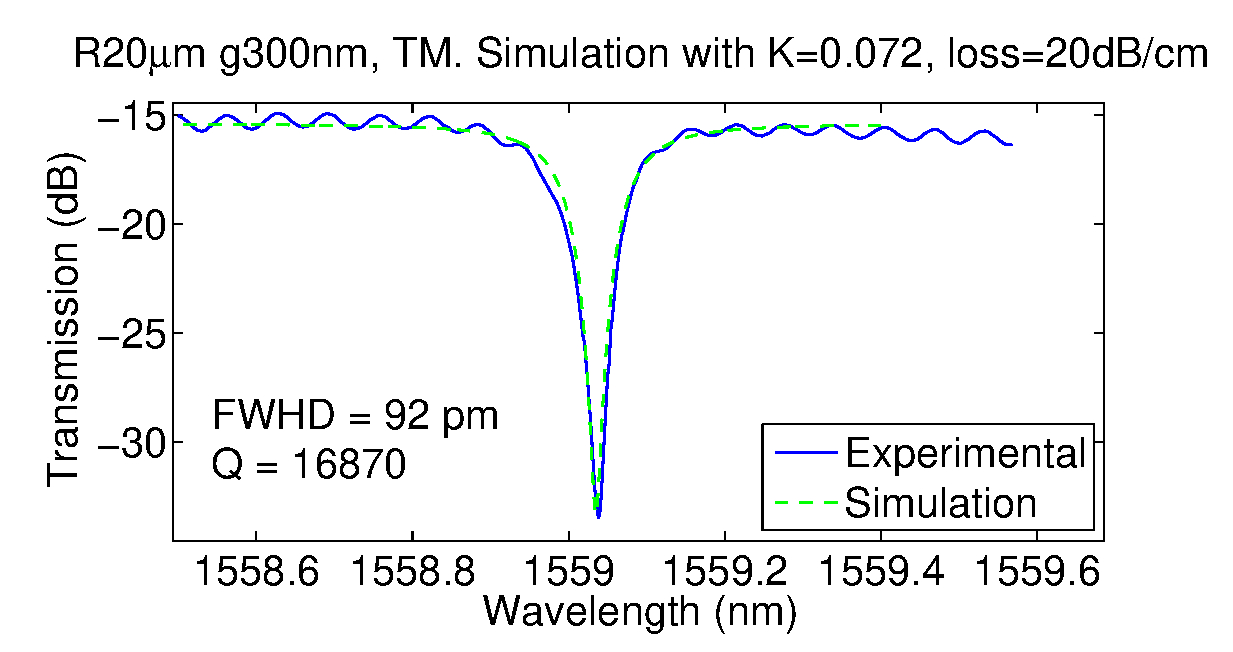
\includegraphics[width=3.5in]{fit20um300nmBig_2}   
    \caption{Transmission spectrum of the ring resonator sample (TM polarization). Solid line is the experimental data and dashed line is the result of the simulation when setting propagation loss to 30~dB/cm and coupling coefficient k = 0.072}
    \label{fig:fit20um300nmBig}
\end{figure}


\section{Experiments}

\subsection{Heterodyne characterization}
In order to study in with great detail the nonlinear effects response, both in phase and module, we used an heterodyne characterization setup. The set up (Fig.~\ref{fig:timeResSetupSwitching}) consists of a series of probe pulses that are affected by a high power pulses (pump). Varying the pump pulses with respect to the probe ones we can see the module and phase response of nonlinear effects such as Kerr, cross absorption modulation and Free-carrier dispersion.


\begin{figure}[htb]
    \centering
    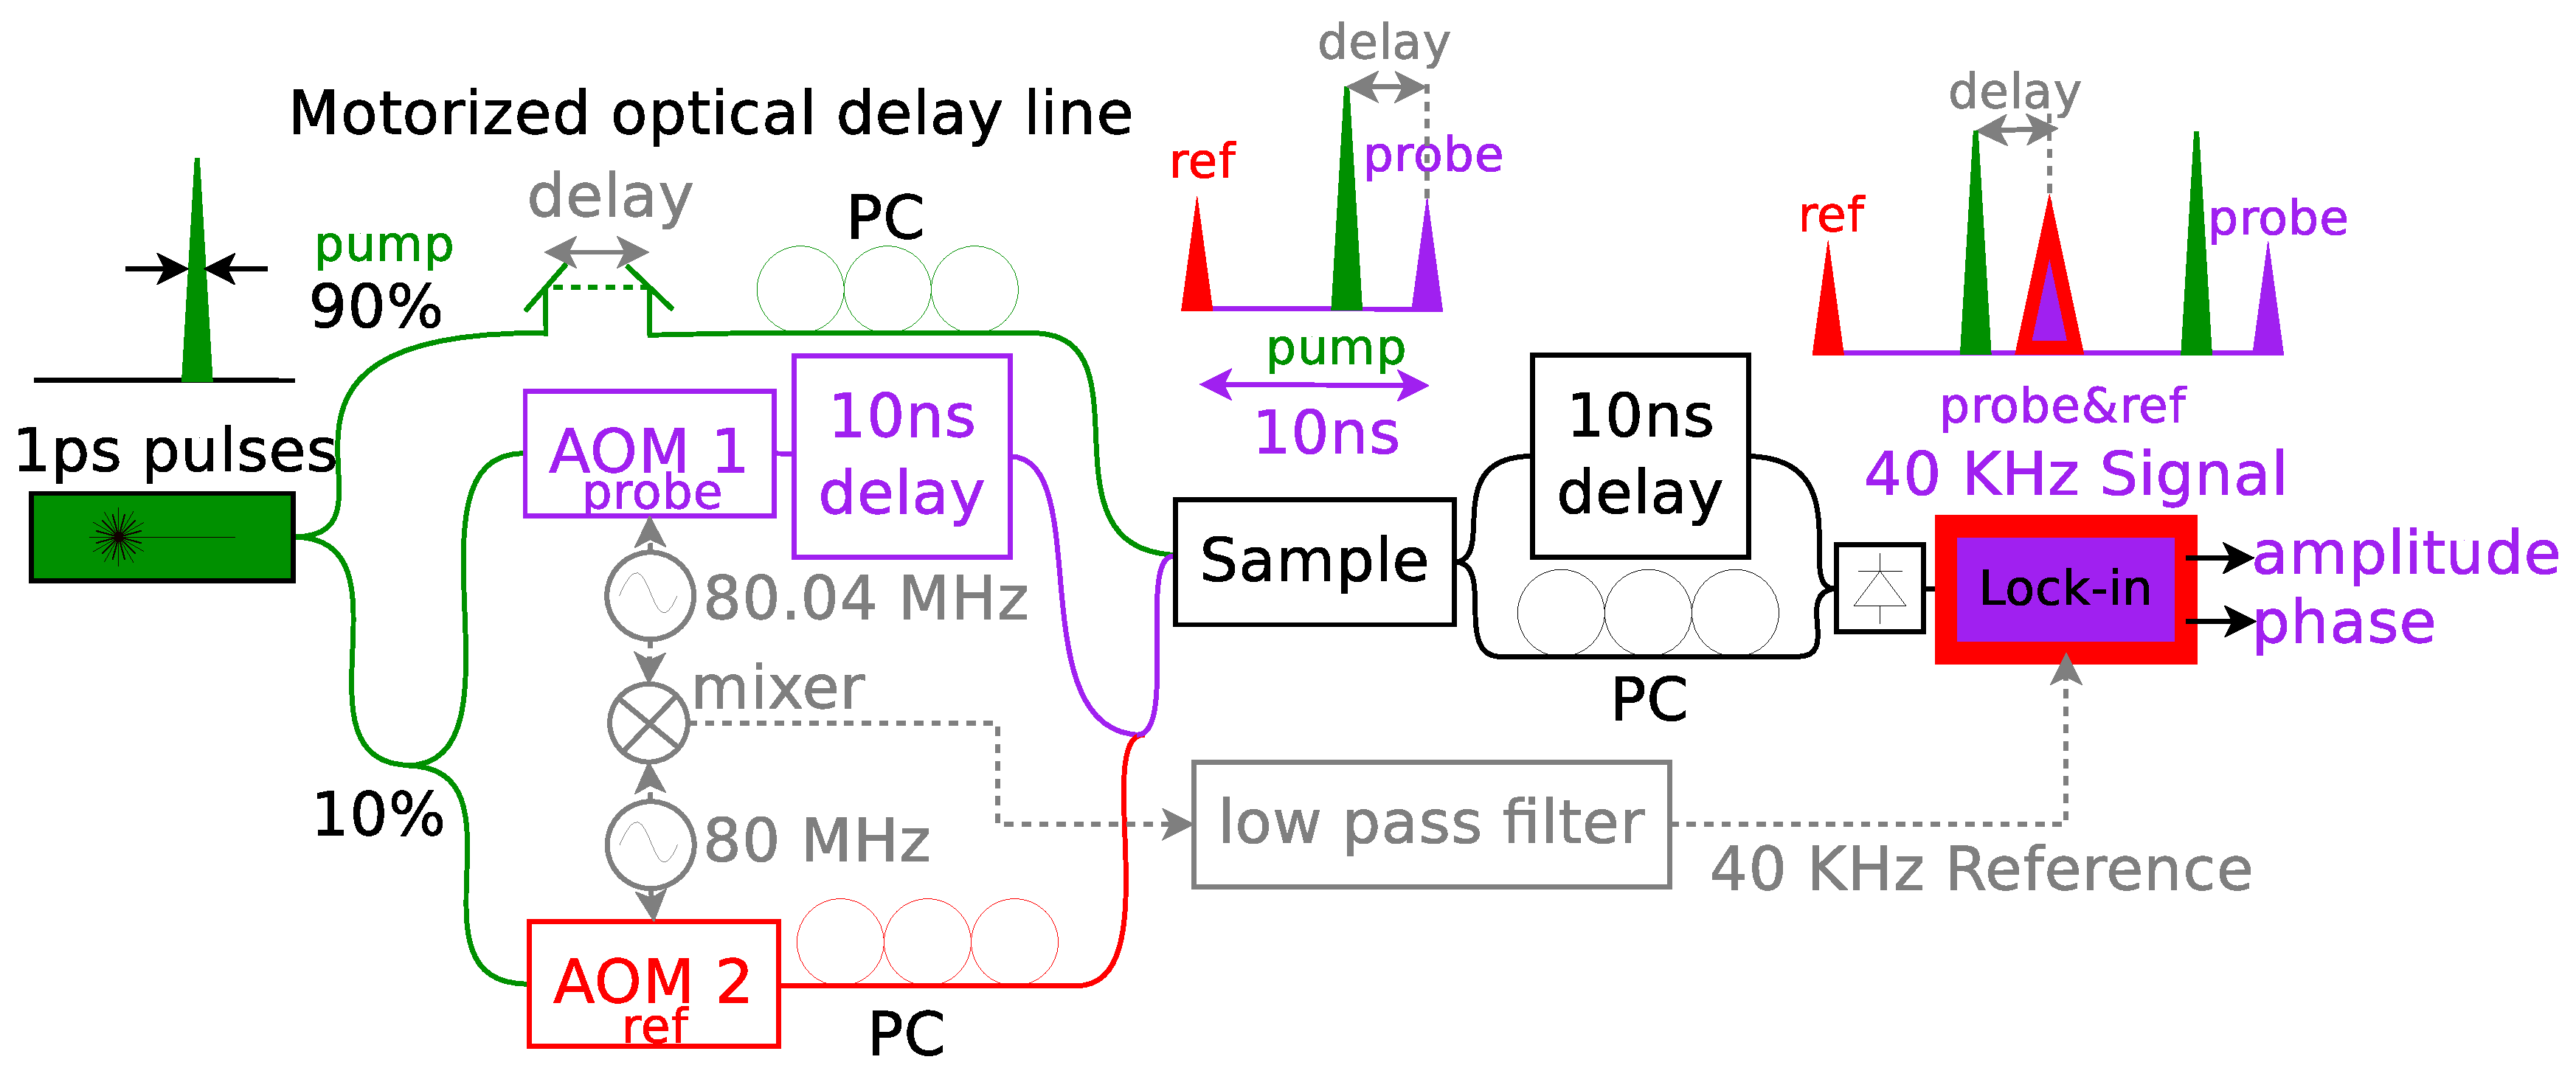
\includegraphics[width=3.5in]{timeResolvedBig}
    \caption{Characterization setup. Blue: RF signals, black: optical signals. Motorized delay line 1 was used to modify the position of the pump pulses respect the probe ones. }
    \label{fig:timeResSetupSwitching}
\end{figure}


The initial pulse is divided into three pulses: two weak ones (a reference and probe separated 10~ns), and one pump pulse, situated close to the probe pulse, and whose temporal position with respect to the probe can be varied. The reference and probe pulses are recombined after passing through the sample, and the beatings they produce are collected in the lock-in. The 40~KHz beatings  are produced because the wavelengths of probe and reference signals are slightly different, as both are shifted with acousto-optic modulators which work at frequencies that only differ by 40~kHz. The amplitude and the phase of the signals are simultaneously monitored.
The amplitude collected is proportional to the amplitude of the probe pulse with respect to the reference, and the phase of the beatings corresponds to the phase shift produced by the pump to the probe pulse, considering the reference pulse as unaffected by the pump, and thus using it as a reference for the phase measurement. 


\subsection{All-optical switching}
The setup for the all-optical switching experiment is shown in Fig.~\ref{fig:switchingSetupSwitching}. A tunable laser was modulated with a LiNbO3 modulator and amplified through Er-doped fiber amplifiers (EDFAs). The pulse train was generated with a 40~Gb/s bit pattern generator, where pulses had 45~ps duration and 6.4~ns period. The peak power coupled into the waveguide was estimated to be 85~mW. A continuous-wave (cw) probe signal was mixed with the pump with a 3~dB coupler and sent to the waveguide through the same fiber with an estimated coupled power of 0.5~mW. Wavelengths of pump and probe signals were respectively 1564 and 1554~nm, chosen to match with two resonances of the micro-ring resonator. The output signal was filtered to remove the pump component and amplified before sending the signal to a 50~GHz photodiode and collecting the data with a 40~GHz sampling scope.


\begin{figure}[htb]
    \centering
    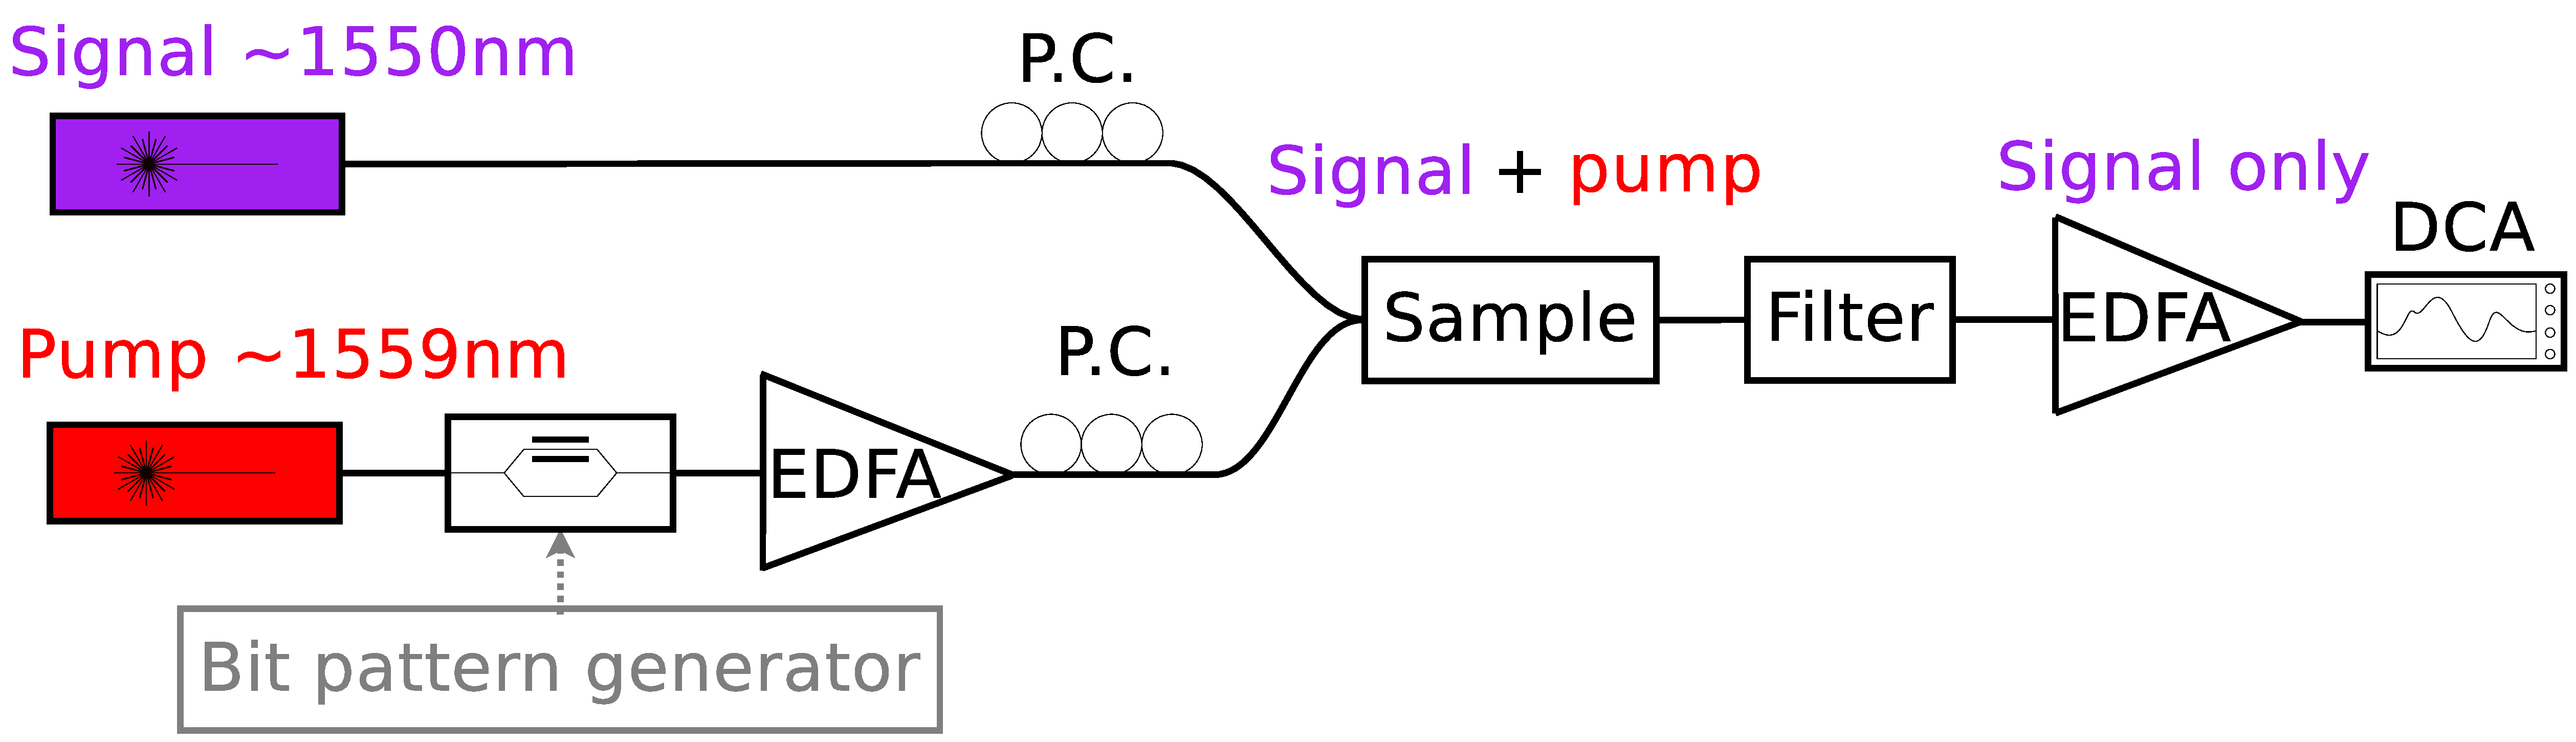
\includegraphics[width=3.5in]{switching}
    \caption{All-optical switching characterization setup. (Triangles represent EDFAs with ASE filters, PC: polarization controllers, DCA: Digital communication analyzer)}
    \label{fig:switchingSetupSwitching}
\end{figure}

\begin{figure}[htb]
    \centering
    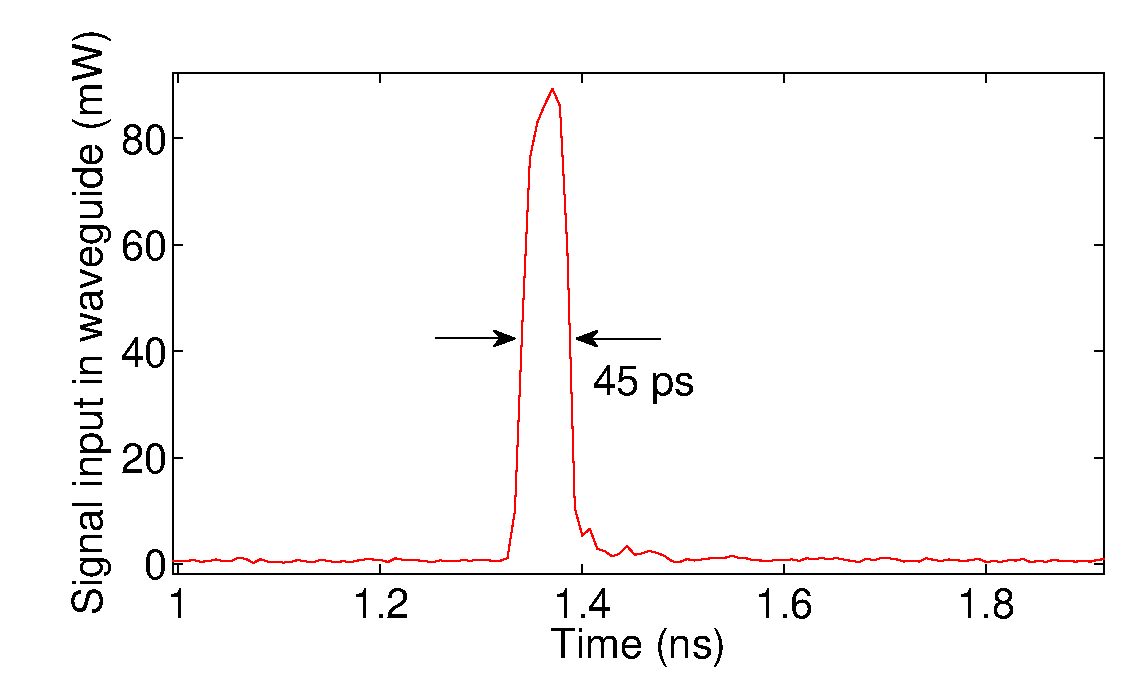
\includegraphics[width=3in]{inputPulsesSwitchingBig}
    \caption{Input pulses with 45~ps duration, 6.4~ns period and 85~mW peak power coupled in the waveguide}
    \label{fig:inputPulsesSwitchingBig}
\end{figure}

\begin{figure}[htb]
    \centering
    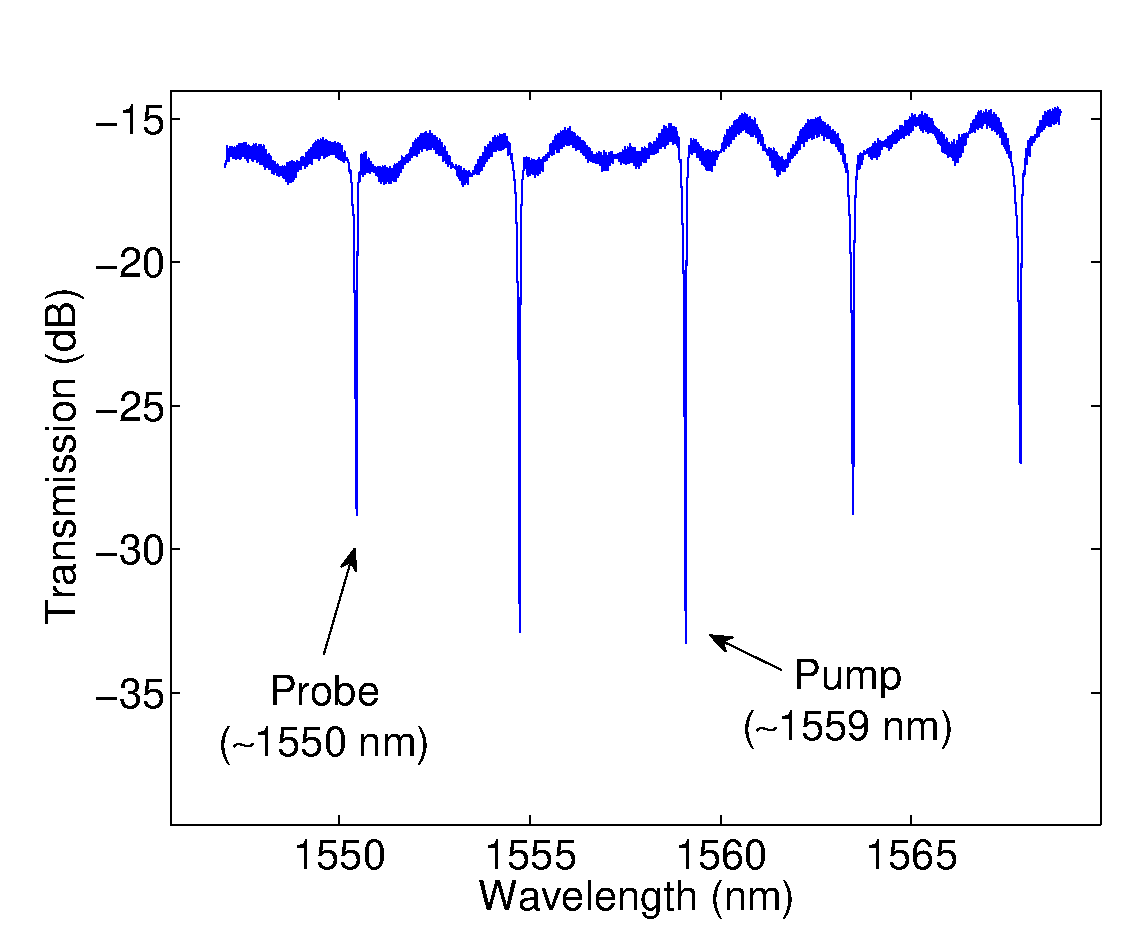
\includegraphics[width=3in]{broadBig}
    \caption{Transmission spectrum of the ring resonator sample (TM polarization). Wavelengths of pump and probe signals were respectively 1564 and 1554~nm.}
    \label{fig:transmissionSwitching}
\end{figure}

\section{Results}
\subsection{Heterodyne experiment}
In Fig.~\ref{fig:ntc02TimeResSwitching} we can see observe both Kerr and carriers effect. They produce opposite phase shifts because Kerr produces an increase in refractive index ($\Delta n > 0$) and carriers decrease it ($\Delta n < 0$).


The dynamics of each of these processes is also very different. During the pump pulse, we can see an instantaneous phase change due to Kerr effect, together with an amplitude decrease. This decrease is due to cross-absorption modulation (XAM), which consists of a two-photon absorption (TPA) process where one of the photons comes from the pump and the other comes from the probe. Once the pump pulse is gone, there is a phase response with opposite sign that remains for more than 100~ps. This is due to the carrier plasma effect, also known as free-carrier dispersion (FCD).

\begin{figure}[htb]
    \centering
    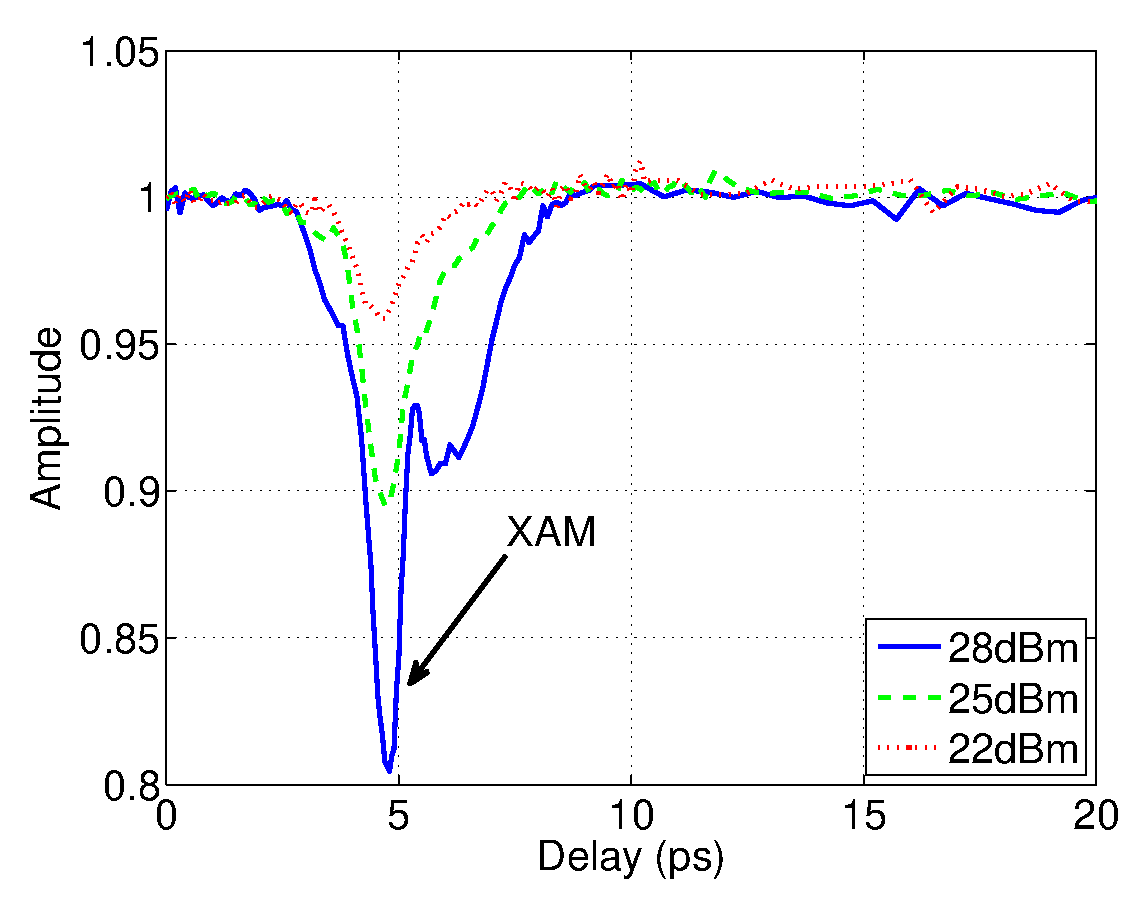
\includegraphics[width=3.5in]{ntc02amp}
    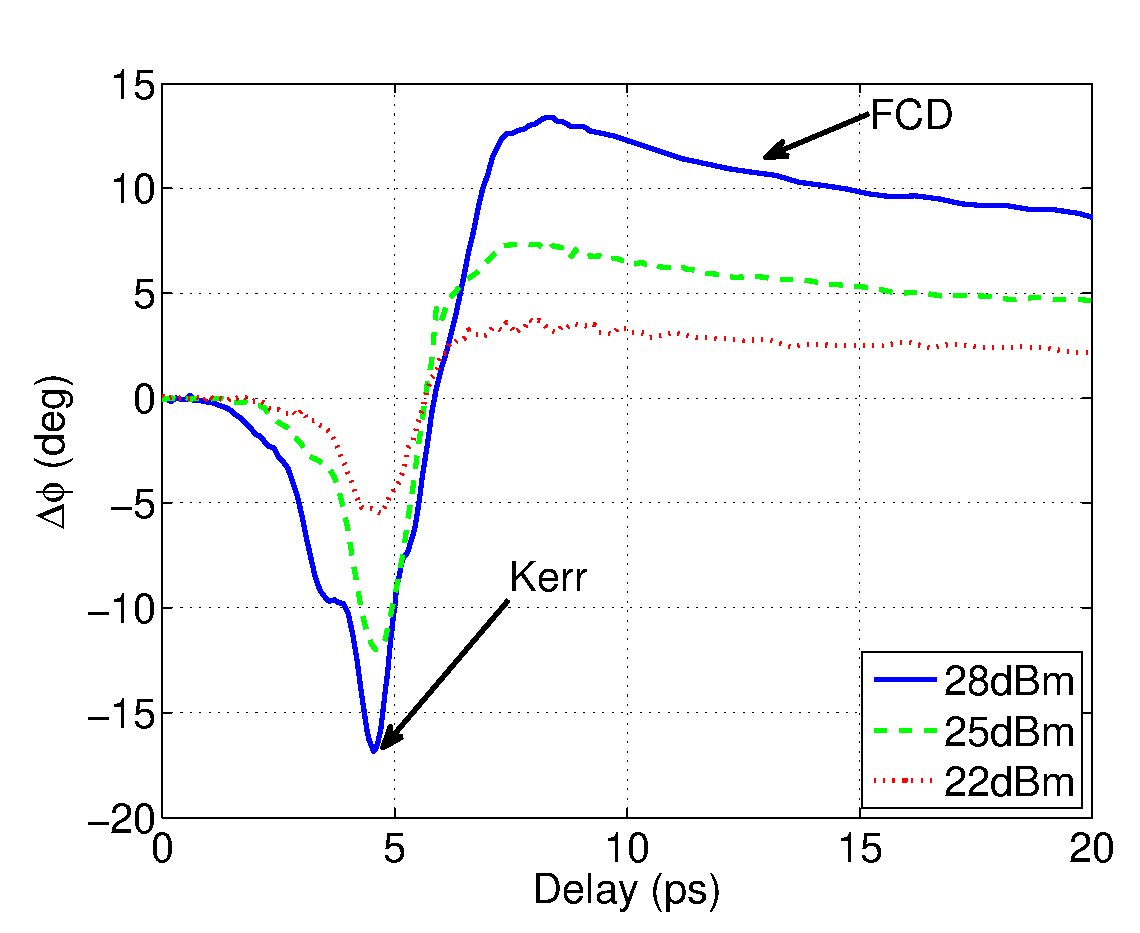
\includegraphics[width=3.5in]{ntc02phase}
    \caption{Sample response for different pump peak powers in the waveguide. Top: phase shift produced in probe pulse versus pump delay time (FCD: Free-carrier dispersion). Bottom: amplitude variation in the probe (XAM: cross absorption modulation).}
    \label{fig:ntc02TimeResSwitching}
\end{figure}

Fitting the carriers decay time to a double exponential, we can clearly observe two tendencies with different recombination times. One of them is very fast (8~ps time constant) whereas the other is much slower (123~ps). (See Fig.~\ref{fig:zoomTimeResNtc02Switching}). Carrier recombination time in Si waveguides is usually reported to be in the ns range \cite{Almeida2004b,Xu2007}, so we attribute this fast response to surface defects in the waveguide.

\begin{figure}[htb]
    \centering
    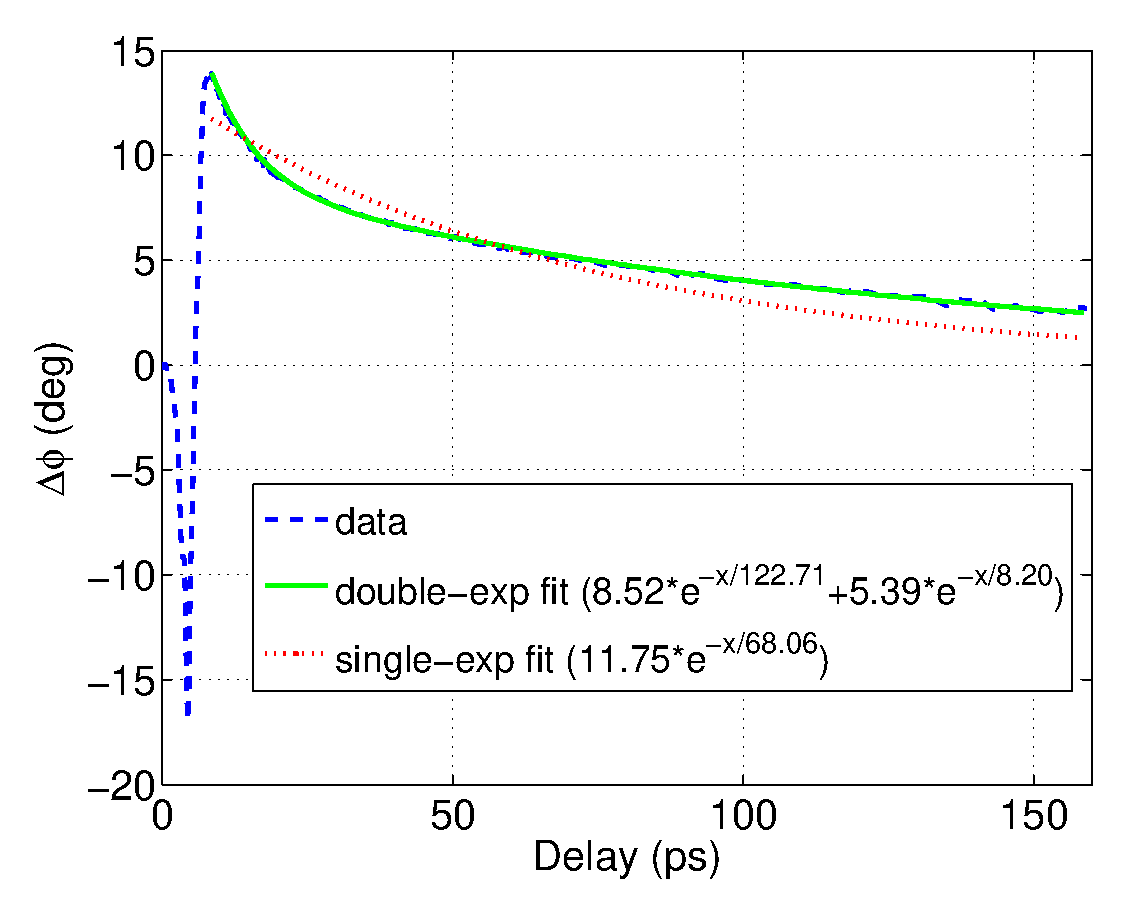
\includegraphics[width=3.5in]{ntc02phase_exp_fit}
    \caption{Panoramic view of the phase response in Fig.~\ref{fig:ntc02TimeResSwitching} showing the free-carriers decay. We use a two-exponential fit to simulate two very different recombination times, as a sigle-exponential fit is not able to follow both tendencies.}
    \label{fig:zoomTimeResNtc02Switching}
\end{figure}


\subsection{Switching experiment}
Figure \ref{fig:ntc02switching} shows the result of the second experiment, which is the demonstration of all-optical switching \cite{Oton}.The carrier dispersion effect produces a phase response, which is converted into intensity modulation by using a micro-ring resonator. As the resonance position blue-shifts when the carriers are excited, and the probe is tuned to the resonance, this shift produces an intensity modulation which is measured with the photo-diode. Using only 85~mW of pump peak power, the extinction ratio is 10.2~dB and the 1/e recovery time is 150~ps, which is close to the decay time observed in the phase-sensitive experiment. Depending on which point of the resonances we tune our CW laser we obtain positive (laser in the minimum of the resonance) or negative pulses (CW laser next to the resonance).  


\begin{figure}[htb]
    \centering
    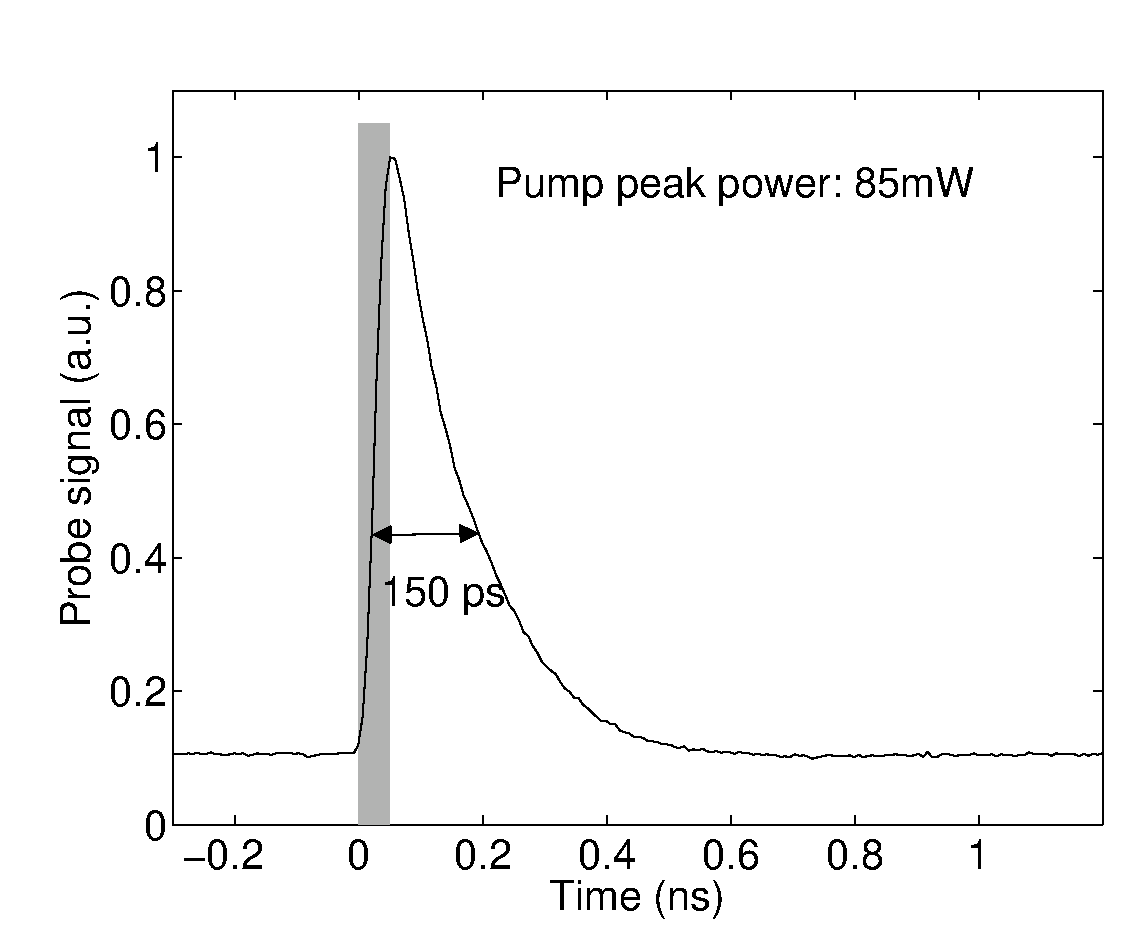
\includegraphics[width=3.5in]{pos_pulse_big}
    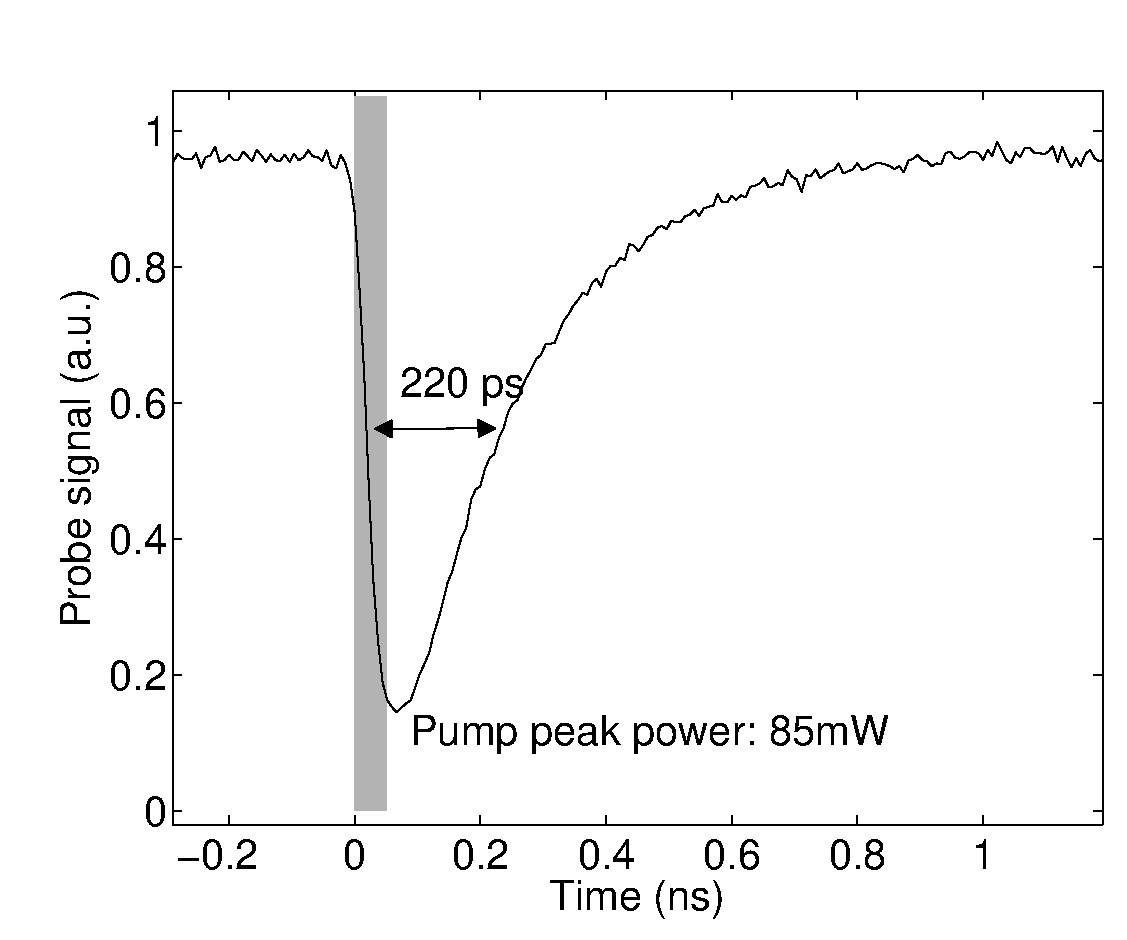
\includegraphics[width=3.5in]{neg_pulse_big}
    \caption{Variation of the probe signal when both pump and probe are resonant with two different modes of the microring. The grey box marks the pump duration. Depending on which point of the resonances we tune our CW laser we obtain positive (left figure) or negative pulses (right figure).}
    \label{fig:ntc02switching}
\end{figure}

\section{Conclusion}
We have characterized the dynamics of the nonlinear response of a Si waveguide with a time-resolved phase-sensitive pump and probe technique. The Kerr and XAM effects are clearly distinguished from the carrier dispersion effect. The carrier decay follows a double exponential decay with constants 8~ps and 122~ps, which is faster than values reported elsewhere. This fast decay time has allowed the fabrication of an all-optical switch with 10~dB extinction ratio and 150~ps recovery time, by using only 85~mW of pump peak power.

\section{Acknowledgements}
This work has been sponsored by the Spanish Science and Innovation Ministry through SINADEC (TEC2008-06333) and DEMOTEC (TEC2008-06360) contracts and by Generalitat Valenciana through PROMETEO-2010-087R\&D Excellency Program (NANOMET).

\bibliographystyle{unsrt}
\bibliography{/home/joaquin/Documents/library}
\end{document}

